\chapter{从 AgentOS 产品到智能基础设施}

\begin{chapteroverviewbox}
本章讨论 AgentOS 从单一智能体产品、开发框架与运行时系统，进一步演化为通用智能基础设施的理论条件与工程边界。这里的“基础设施”并不意味着 AgentOS 替代 Linux、云计算平台、数据库或基础模型，而是意味着：当持续智能体成为一种长期运行的软件主体以后，传统计算机操作系统仅管理 CPU、内存、设备、文件和网络已经不足以覆盖新的系统对象；还必须有一层长期负责认知状态、生命周期记忆、技能、身体、工具、权限、身份、跨 Agent 协作以及智能资源调度的运行时。因此，本章把 AgentOS 定义为一种 \emph{Intelligence Resource Runtime}，并进一步研究它如何通过 Memory Ecosystem、Skill Ecosystem、Body Ecosystem、Agent Communication、Organization Runtime 与开放标准形成新的软件基础设施。本章仍然以此前确定的固定核心功能拓扑 AgentOS 为主要工程对象，不把任意自修改拓扑作为既定工程能力；所有生态扩展都必须服从单一持续主体、现实验证、权限边界、安全治理以及 ``Computer OS 管理计算资源，AgentOS 管理智能资源'' 的基本分层原则。
\end{chapteroverviewbox}

\begin{figure}[htbp]
\centering
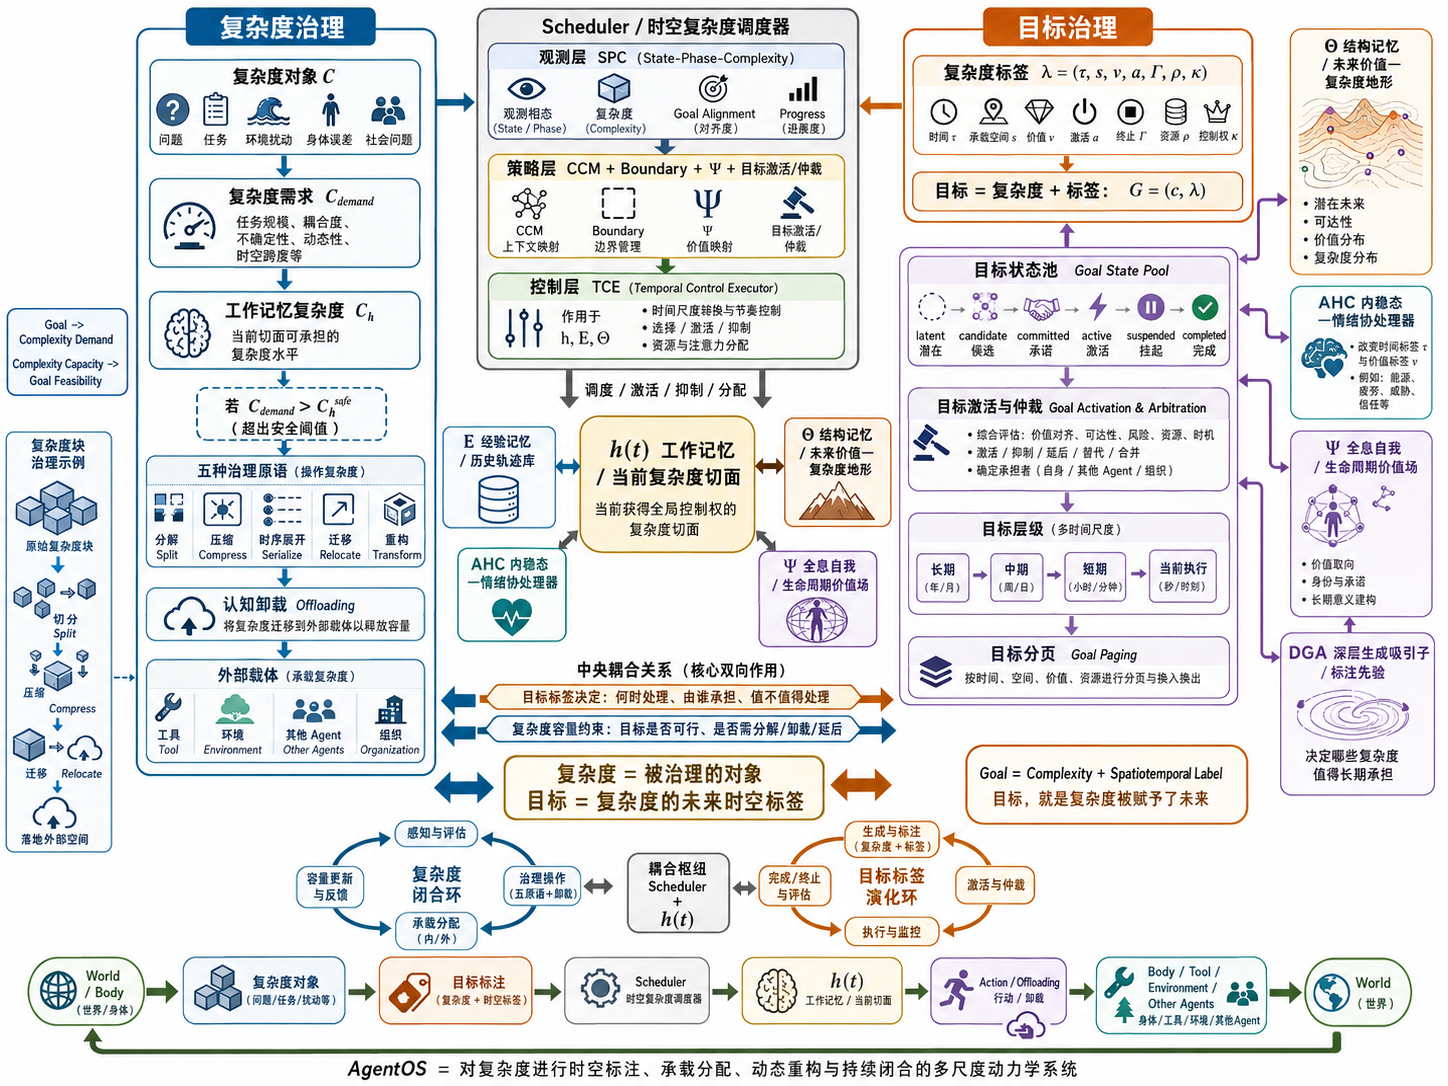
\includegraphics[width=.9\textwidth,height=.38\textheight,keepaspectratio]{images/global-local-predictive-control.png}
\caption{从 AgentOS 产品到智能资源运行时}
\end{figure}
\section{从应用框架到持续智能运行时}

我们首先需要澄清一个容易被工程实现掩盖的问题：AgentOS 最初看起来很容易被理解成一种 ``Agent Framework''。如果仅观察它的表面接口，这种理解并非毫无根据。AgentOS 同样需要调用基础模型、管理工具、维护 Memory、执行任务、响应事件，并与数字世界或物理身体交互。从传统软件工程视角看，这些能力似乎完全可以被组织成若干 SDK、服务组件和工作流。因此，一个最自然的问题是：为什么还需要使用 ``OS'' 这一名称，而不能把它归入普通 Agent Framework、Workflow Engine 或 Application Runtime？

关键区别并不在于组件数量，而在于系统所管理对象的性质发生了变化。普通应用框架通常假定应用本身是短生命周期、可重启、可复制甚至可随时销毁的计算对象，其核心任务是帮助开发者更方便地调用已有资源。AgentOS 所面对的对象却是一个具有生命周期连续性的智能主体。我们此前已经规定，在主体层 $D_1$ 上需要保持
\[
N_{\mathrm{Agent}}^{D_1}=1,
\]
并进一步约束
\[
fork(A)=\mathrm{Forbidden},\qquad
new(A)=\mathrm{Forbidden},\qquad
delete(A)=\mathrm{Forbidden},
\]
这里并不是从操作系统层面禁止创建普通进程，而是要表达一个更深的语义约束：属于同一个生命周期的持续主体不能被当作普通 worker 任意复制。任务、线程、工具调用和局部 worker 可以大量存在，但它们并不自动拥有主体地位。由此可见，AgentOS 所管理的不只是执行流，而是一个具有历史、身份、记忆、能力和权限积累的持久过程。

因此，我们可以把传统应用框架抽象为
\[
\mathcal F_{\mathrm{app}}
=
(\mathcal T,\mathcal R,\mathcal API),
\]
其中 $\mathcal T$ 是任务集合，$\mathcal R$ 是计算资源，$\mathcal API$ 是外部接口；而持续 Agent Runtime 至少需要表示
\[
\mathcal A(t)
=
\bigl[
h(t),E(t),\Theta(t),\Psi(t),\Omega(t),
G(t),B(t),K(t),\mathcal M_{\mathrm{ext}}(t)
\bigr],
\]
其中 $h$ 为工作记忆状态，$E$ 为情景轨迹，$\Theta$ 为长期生成结构，$\Psi$ 为自我与身份慢变量，$\Omega$ 为生命周期生成吸引子，$G$ 为目标结构，$B$ 表示身体及身体接口状态，$K$ 表示技能集合，$\mathcal M_{\mathrm{ext}}$ 表示被主体组织起来的外部认知载体。这样一来，任务执行就不再是孤立映射
\[
Task\rightarrow Result,
\]
而成为
\[
\mathcal A(t)
\xrightarrow{\mathrm{Task}}
\mathcal A(t+\Delta t),
\]
也就是说，每一次任务都有可能改变未来的主体。

这使 AgentOS 从传统软件栈中的 ``任务工具箱'' 转变为一个管理持续智能状态演化的 Runtime。它关心的不是某次 API 调用是否成功，而是一次成功或失败如何写入 $E$，是否需要改变 $\Theta$，是否影响 $\Psi$，是否使某个技能成熟，是否改变未来 Boundary 策略，以及是否需要调整 Agent 可获得的权限和自治水平。于是，AgentOS 的核心操作对象不再只是文件、线程和进程，而逐渐扩展为
\[
\boxed{
Goal,\;
AgentCSO,\;
Memory,\;
Skill,\;
Body,\;
Tool,\;
Authority,\;
Lifecycle
}.
\]

这里必须特别强调：把 AgentOS 称为 ``OS'' 并不意味着它应该重新实现 Linux 内核。相反，我们一直坚持
\begin{statementbox}
\centering
\adjustbox{max width=.96\linewidth}{\(\displaystyle Hardware
\rightarrow
ComputerOS
\rightarrow
AgentOS\)}
\end{statementbox}
这一分层结构。Linux 负责计算现实的稳定抽象，例如进程、虚拟内存、设备、文件和网络；AgentOS 则建立在这些抽象之上，把它们重新组织成对长期智能体有意义的认知资源。因此，可以作如下功能区分：
\[
\boxed{
ComputerOS=\text{Compute Resource Runtime}
}
\]
以及
\[
\boxed{
AgentOS=\text{Intelligence Resource Runtime}.
}
\]

前者回答的是 ``计算资源如何安全、高效地分配''，后者回答的是 ``有限认知能力应该在生命周期中如何分配、沉降、外化和恢复''。这一转换构成 AgentOS 从产品走向基础设施的第一步：只有当管理对象从应用调用上升为持续智能资源时，系统才具有形成独立基础设施层的理论必要性。

\section{智能资源：AgentOS 基础设施层真正管理什么}

如果 AgentOS 要成为基础设施，就必须进一步回答一个操作系统意义上的问题：它究竟在管理什么资源？传统计算机操作系统之所以能够成为基础设施，是因为它建立了对有限计算资源的稳定抽象。例如 CPU 时间被抽象为进程和调度片，物理内存被抽象为虚拟地址空间，块设备被抽象为文件系统，网络硬件被抽象为 socket。相应地，如果 AgentOS 只是把若干 Prompt、Tool 和 Memory 包装起来，它仍然不足以形成新的基础设施层。它必须形成属于智能自身的一组稳定资源抽象。

我们可以从工作记忆有限性出发建立这一资源理论。此前已经提出，在任意时刻，Agent 可以稳定维持的显式认知结构受到上界约束：
\[
C_{\mathrm{run}}(t)\leq C_{\max}(W).
\]
这里 $W$ 不是固定 token 个数，而是当前系统能够在 $h(t)$ 中维持的有效关系结构容量。该约束意味着：持续智能的第一种稀缺资源不是磁盘，而是 \emph{显式全局认知带宽}。于是，AgentOS 的第一个核心资源可以表示为
\[
R_h(t)=\text{AvailableExplicitCognitiveCapacity}.
\]
CCM、Scheduler、Boundary 和 Offloading 的存在，本质上都是围绕这一稀缺资源展开的。CCM 防止当前认知关系超过容量，Scheduler 决定哪些目标与任务获得当前认知时间，Boundary 决定什么信息有资格进入，Offloading 则把不需要持续占据 $h$ 的结构迁移到更适合的载体。

第二类资源是记忆稳定度。一个认知结构并不只有 ``存在/不存在'' 两种状态，而可能分别承载在
\[
h,\quad E,\quad \Theta,\quad \Psi,\quad \Omega
\]
不同时间尺度之中。因此，AgentOS 管理的实际上是不同结构稳定度上的认知存储。可以把某个 Agent-CSO $C_i$ 的承载状态表示为
\[
\chi_i(t)
=
(R_i,F_i,\tau_i,B_i,S_i),
\]
其中 $R_i$ 是具体表示方式，$F_i$ 是当前功能承载，$\tau_i$ 是有效时间尺度，$B_i$ 是内部或外部边界位置，$S_i$ 表示激活状态。学习的许多过程都可以被理解为 $\chi_i$ 的变化，而 AgentOS 的责任就是确保这种变化不会破坏主体连续性。

第三类资源是技能。Skill 不应被理解为任意一个外部函数。我们此前将成熟技能定义为一种经过重复认知而逐渐沉降形成的局部闭环：
\[
\boxed{
BodySkill
=
LocalPredictor
+
LocalController
+
ResidualModel.
}
\]
对于数字 Agent，这个 ``BodySkill'' 可以表现为稳定脚本、浏览器操作程序、工具组合或者局部 policy。对于具身 Agent，它可能是移动、抓取、操作设备等身体闭环。Skill 因而是一种被编译后的认知资本：它减少未来相同问题再次占用 $h$ 的必要性。于是可以定义技能资本
\[
K_A(t)=\{k_1,k_2,\ldots,k_n\},
\]
并用执行成本、成功率、残差分布、适用条件和权限边界描述每个技能。

第四类资源是身体能力。Body 并不是外围设备，而是主体可观察和可控制现实的有效边界：
\[
\boxed{
Body
=
ControlledAndSensedCarrierOfAgency.
}
\]
因此，AgentOS 还必须维护某种能力集合
\[
\mathcal C_B(t)
=
\{
c^{percept}_i,
c^{control}_j,
c^{predict}_k,
c^{safety}_l
\}.
\]
换句话说，Agent 并不是抽象地 ``拥有世界''，而是只能通过当前身体访问一个有限的可观测和可行动子空间。Body Scale 理论正是在讨论这种能力能否在不同身体之间迁移。

第五类资源是权限与自治。传统 OS 权限往往是静态 ACL 或 capability；持续 Agent 中，权限还具有生命周期含义。Agent 的能力、信任和自治程度可能随长期经验变化：
\[
Experience
\rightarrow
Capability
\rightarrow
Evaluation
\rightarrow
Authority
\rightarrow
Autonomy.
\]
因此，权限不是简单安全配置，而成为一种慢尺度认知资源。AgentOS 必须明确哪些资源可以被主体自主访问，哪些只能经治理层授权，哪些能力可以在成长过程中逐步解锁。

综合来看，我们可以把 AgentOS 管理的智能资源定义为
\[
\mathcal R_I(t)
=
\Bigl[
R_h,
\mathcal M,
K,
\mathcal C_B,
\mathcal T_{\mathrm{tool}},
\mathcal A_{\mathrm{authority}},
\mathcal B_{\mathrm{boundary}}
\Bigr],
\]
其中 $\mathcal M$ 表示多时间尺度记忆，$K$ 表示技能资本，$\mathcal C_B$ 表示身体能力，$\mathcal T_{\mathrm{tool}}$ 表示工具资源，$\mathcal A_{\mathrm{authority}}$ 表示权限和自治，$\mathcal B_{\mathrm{boundary}}$ 表示当前可访问世界与认知边界。AgentOS 因而不再是 ``帮助模型调用工具的软件''，而是在有限主体约束下持续调度
\begin{remark}
认知容量、记忆稳定性、技能、身体能力、外部结构与自治权限
\end{remark}
的系统。这种资源抽象一旦稳定，AgentOS 才真正具有成为基础设施的条件。

\section{Memory Ecosystem：从记忆模块到跨载体认知结构体系}

当 AgentOS 走向基础设施后，Memory 首先会从单一产品内部模块扩展成生态。传统 Agent Memory 往往采用 ``向量数据库 + 摘要 + 对话历史'' 的形式，因此所谓记忆生态容易被误解成 ``支持更多数据库后端''。但按照三相记忆和 CSO 迁移理论，Memory Ecosystem 的核心问题并不是数据存在哪里，而是：一个 Agent-CSO 应该以何种稳定度、何种形式、何种索引关系和何种修改成本被长期承载。

内部记忆最基本的结构为
\[
\mathcal M_{\mathrm{int}}
=
(h,E,\Theta,\Psi,\Omega),
\]
其中 $h$ 是当前显式状态，$E$ 是情景轨迹，$\Theta$ 是结构与生成记忆，$\Psi$ 是身份和价值慢结构，$\Omega$ 是生命周期生成吸引子。但真实 Agent 的长期认知体系远远不止内部记忆。我们此前已经把 Script、Skill、File、Database、Program、Tool、Environment 和 Other Agent 都纳入广义外部承载体系。因此更完整的记忆关系应写为
\[
\mathcal M_A
=
\mathcal M_{\mathrm{int}}
\bowtie
\mathcal M_{\mathrm{ext}},
\]
其中
\[
\mathcal M_{\mathrm{ext}}
=
\{
File,DB,Program,Skill,Tool,Environment,OtherAgent
\}.
\]

需要特别注意，并非外界中所有东西都是 Agent 的记忆。一个文件只有在 Agent 建立了可靠的索引、语义关系、权限路径和恢复机制后，才成为其认知体系中的有效外部承载。因此可以定义一个外部记忆关系
\[
m_j^{ext}
=
(C_j,L_j,I_j,R_j,P_j),
\]
其中 $C_j$ 表示所承载 CSO，$L_j$ 表示外部位置，$I_j$ 是可恢复索引，$R_j$ 是重建或读取规则，$P_j$ 是访问权限。若缺少 $I_j$ 或 $R_j$，即使物理数据存在，也不能认为它属于 Agent 的有效记忆。

这一点使 Memory Ecosystem 的设计目标发生根本变化。它不是追求 ``尽可能记住更多''，而是优化一个跨载体结构配置问题：
\[
\min_{\mu}
\int
\left[
\lambda_h C_h(t)
+
\lambda_r C_{\mathrm{retrieval}}(t)
+
\lambda_m C_{\mathrm{modification}}(t)
+
\lambda_l L_{\mathrm{loss}}(t)
\right]dt,
\]
其中 $\mu$ 表示 Agent-CSO 到不同记忆载体之间的配置映射，$C_h$ 是持续占用工作记忆的代价，$C_{\mathrm{retrieval}}$ 是未来检索代价，$C_{\mathrm{modification}}$ 是修改成本，$L_{\mathrm{loss}}$ 则是结构丢失或失真的风险。不同类型的结构应该选择不同的载体。例如短期未决结构应停留在 $h$ 或近期 $E$；重复经验可能形成 $\Theta$；稳定操作过程可能沉降成 Skill；高精度事实资料更适合数据库或文件；需要世界直接参与维持的状态则可能通过环境结构保存。

这使认知卸载得到更严格的含义：
\[
\boxed{
Offloading
=
AgentCSOCarrierMigration
}
\]
而不是简单地 ``把内容写出 Context''。有效卸载必须保证：
\[
Recoverability>0,\qquad
SemanticLinkage>0,\qquad
FutureUtility>Cost.
\]
否则，所谓卸载只是一种遗忘。

Memory Ecosystem 因而需要开放而稳定的标准，使不同外部存储、数据库、知识系统、文件系统和工具能够被 AgentOS 以统一语义组织。这里并不要求所有 Memory Provider 使用同样的内部实现，而要求至少能够回答：这个载体保存什么结构、可信度如何、更新时间是多少、读取与修改成本如何、是否允许主动写入、是否支持版本和撤销、它与当前主体的关系是什么。换言之，AgentOS 对外部 Memory 的要求不是统一数据库，而是统一认知契约。

从基础设施视角看，这一点十分关键。传统 OS 通过文件系统把不同磁盘抽象成统一文件接口；AgentOS 则需要把不同认知载体抽象成一种更高层的 ``可恢复结构空间''。未来某个 Agent 可能同时使用本地结构记忆、个人数据库、组织知识库、网络文件、工具状态乃至另一个 Agent 的专业能力，而 AgentOS 应负责维持它们与主体内部 CSO 图之间的稳定关系。Memory Ecosystem 因此不是附属插件市场，而是持续智能得以突破单体模型容量限制的第一层基础设施。

\section{Skill Ecosystem：把过去的推理沉降为未来的能力}

如果 Memory Ecosystem 解决的是 ``结构如何跨时间保存''，那么 Skill Ecosystem 解决的则是 ``过去的高成本认知如何转化为未来低成本能力''。这一点是 AgentOS 与传统知识型 Agent Framework 之间非常重要的区别。一个不具有技能沉降机制的 Agent，即使保存了大量过去经验，也可能在每一次重复任务中重新调用 LLM、重新规划和重新探索。它记得自己做过，却没有真正变得熟练。

我们此前已经给出技能形成的基本结构：
\[
ExplicitCognitiveControl
\rightarrow
RepeatedTrajectory
\rightarrow
StablePolicy
\rightarrow
CompiledSkill.
\]
从 CSO 理论看，这个过程可以进一步解释为 Agent-CSO 的功能与时间尺度迁移：
\[
AgentCSO(C;F_{high},\tau_{slow})
\rightarrow
AgentCSO(C;F_{local},\tau_{fast}).
\]
也就是说，同一个任务相关结构原先需要通过 $h$、规划器和高层模型显式处理，经过大量稳定经验后，逐渐迁移到局部闭环。系统成熟的一个重要标志不是 ``每次都想得更多''，而是
\begin{statementbox}
\centering
\adjustbox{max width=.96\linewidth}{\(\displaystyle \frac{ExplicitCognitiveIntervention}
{SuccessfulRoutineBehavior}
\downarrow.\)}
\end{statementbox}

因此，Skill Ecosystem 不能退化成传统意义上的 ``函数商城''。一个真正意义上的 Skill 至少需要具备能力描述、适用条件、状态前提、权限要求、执行接口、成功判定、残差返回、风险边界和版本信息。可以把技能描述为
\[
k_i
=
(
Pre_i,
Cap_i,
Policy_i,
Post_i,
Residual_i,
Risk_i,
Authority_i
).
\]
其中 $Pre_i$ 描述可执行前提，$Cap_i$ 是能力语义，$Policy_i$ 是内部实现，$Post_i$ 是预期后验状态，$Residual_i$ 描述执行偏差，$Risk_i$ 是风险模型，$Authority_i$ 则确定调用权限。只有这样，Skill 才可以安全进入 AgentOS 的认知调度体系。

这里需要特别区分 ``调用 Skill'' 与 ``相信 Skill''。一个 Skill 即使长期稳定，也不能拥有对现实状态的最终解释权。仍然必须遵守
\[
\boxed{
ActionIssued\neq ActionSucceeded
}
\]
以及
\begin{statementbox}
RealityIsUltimateConstraint.
\end{statementbox}
因此，Skill 执行后的实际结果必须重新通过 Body Runtime、工具返回值或者其他 Reality Interface 进入 AgentOS，再由 SGC、FCS 或相应数字语义接口形成真实观测。只有这样，Skill 才不会成为一个把预测状态偷偷写回现实状态的封闭环。

Skill Ecosystem 还提供了跨 Agent 共享能力的基础。设 Agent $A$ 已经学习某 Skill $k_A$，Agent $B$ 若具有相容身体能力和接口，则可以尝试把该 Skill 迁移为
\[
\mathcal T_{A\rightarrow B}(k_A)
=
k_B.
\]
这里 $\mathcal T$ 不应只是文件复制，而需要验证 Body Capability、SGC/FCS 语义、ControlReference、权限与风险条件是否相容。因此 Skill 的真正可移植性与 Body Scale 密切相关：
\[
\fitdisplay{
Transferability(k)
=
F(
SemanticCompatibility,
BodyCompatibility,
ControlCompatibility,
SafetyCompatibility
).
}
\]

当 Skill 成为开放生态后，AgentOS 将发生类似传统软件从 ``每个应用自己实现功能'' 向 ``标准库、包管理器和服务生态'' 的跃迁。但这里必须比普通软件包管理更严格，因为 Skill 是行动能力，而不仅是静态代码。Skill 的安装意味着 Agent 的可行动空间发生变化：
\[
\mathcal A_{action}^{t+1}
=
\mathcal A_{action}^{t}
\cup
\Delta \mathcal A_k.
\]
因此，每个 Skill 的加入本质上也是权限和主体能力边界的扩张。

由此，Skill Ecosystem 的基础设施意义可以明确表述为：它使文明中已经被某些 Agent 高成本学习完成的认知过程，能够被编译、封装、验证并迁移给其他 Agent。其结果不是简单的软件复用，而是
\begin{statementbox}
\centering
\adjustbox{max width=.96\linewidth}{\(\displaystyle PastCognition
\rightarrow
SharedExecutableCapability.\)}
\end{statementbox}
这使 AgentOS 的成长机制第一次突破单一主体的生命周期限制：个体经验可以沉降为技能，技能可以进入生态，生态又成为后来 Agent 的初始能力空间。由此，技能不再只是产品功能，而成为智能社会中的可积累基础资本。

\section{Body Ecosystem：让同一个主体进入不同现实}

如果 Memory Ecosystem 扩展了 Agent 的时间边界，Skill Ecosystem 扩展了能力边界，那么 Body Ecosystem 扩展的则是主体的现实边界。Body 在我们的理论中从来不等于机械身体，而被定义为
\[
\boxed{
Body
=
ControlledAndSensedCarrierOfAgency.
}
\]
因此，浏览器、桌面操作系统、Shell、文件系统、机器人、汽车和人形身体都可以成为不同形式的 Body。真正重要的问题不是它们物理形态是否一致，而是 Agent 能否通过稳定接口获得感知、功能影响、预测和控制能力。

Body Scale 理论已经给出一个重要判断：
\[
\boxed{
BodyScale
=
PerceptualTransfer
+
FeelingTransfer
+
PredictiveTransfer
+
ControlTransfer.
}
\]
一个 Agent 是否具有大 Body Scale，不取决于它控制的机器有多大，而取决于同一个认知 Kernel 在切换身体以后，可以保留多少既有意义、世界模型、技能与控制结构。理想状态不是每换一个 Body 就重新训练一个完整智能体，而是
\[
KnownMeaning
+
NewBodyGrounding
\rightarrow
NewEmbodiment.
\]

为实现这一点，我们把 Body Runtime 设计成相对独立的高频运行层：
\[
\boxed{
AgentSystem
=
AgentKernel
\bowtie
BodyRuntime.
}
\]
Kernel 决定 ``做什么''，Body Runtime 负责 ``这个身体怎样做到''。两者之间通过 FBI、SGC、FCS、ControlReference、PredictiveEnvelope、BPCCFeedback 和 Safety 等稳定语义接口交互。由此，Body Ecosystem 的核心不再是统一机器人硬件，而是统一 ``主体如何理解一个身体''。

SGC 在这里提供可行动现实的语义结构：
\[
SGC
=
Geometry
+
Entity
+
Relation
+
Affordance
+
EpistemicMetadata,
\]
回答
\begin{statementbox}
WhatIsThere?
\end{statementbox}
而 FCS 提供世界与身体对主体的功能影响：
\[
FCS
=
TypedInfluenceField,
\]
回答
\begin{statementbox}
HowIsRealityAffectingMe?
\end{statementbox}
两者共同构成公开的具身语义状态。BPCC 则保留高频局部预测控制：
\[
BPCC
=
FastPrediction
+
FastControl
+
ResidualEstimation
+
AdaptiveLearning.
\]
这样，Agent Kernel 就不必直接面对每个电机、电池、光标或浏览器 DOM 的所有细节。

Body Ecosystem 因此需要一种类似设备生态但更高级的能力描述。例如，一个 Body Provider 至少应该暴露
\[
BodyCapabilityDescriptor
=
(
Perception,
Action,
Timescale,
Accuracy,
Risk,
Safety,
Resource
).
\]
其中 Perception 表示可感知结构类型，Action 表示可执行动作空间，Timescale 表示控制频率，Accuracy 表示感知与控制误差，Risk 表示潜在伤害，Safety 表示不可覆盖保护机制，Resource 表示能源、算力或其他运行约束。AgentOS 通过这一 Capability Descriptor 才能判断：一个 Goal 是否在当前身体上可实现，某 Skill 是否可迁移，某 ControlReference 是否会超过身体安全能力。

Body Ecosystem 的出现还会改变机器人产业的软件分层。传统机器人软件往往围绕具体硬件构建完整 stack，感知、规划、控制和任务逻辑高度耦合。AgentOS 的目标则是让认知 Kernel 与具体身体相对解耦：
\[
\frac{\partial Architecture_{\mathrm{Kernel}}}
{\partial Body_i}
\rightarrow 0.
\]
这里并不是要求完全零依赖，而是使 Body 差异主要被 Body Runtime 和 KRA 吸收，而高层认知保持相对稳定。KRA 则负责不同 Body Runtime 与 Kernel 之间持续的语义和动力学校准：
\[
KRA:
BodySemanticSpace
\leftrightarrow
KernelInternalRepresentation.
\]

一旦这一结构成立，同一个持续主体就可能从 Computer Use 身体逐渐扩展到移动操作平台，再进入家庭机器人、车辆甚至人形身体，而不需要每一次重新建立新的 ``自我''。这正是 Body Ecosystem 的基础设施价值：它把现实世界中异构设备转化为 Agent 可继承、可学习、可比较的身体能力空间。

因此，未来 AgentOS 的生态竞争不会只是 ``支持多少设备''，而会逐渐转变成 ``有多少身体能够以统一语义被长期智能主体安全接入''。在这一层面上，Body Driver 与传统 Device Driver 的区别是根本性的：Device Driver 解决硬件访问，而 Body Driver 解决的是
\begin{statementbox}
\centering
\adjustbox{max width=.96\linewidth}{\(\displaystyle HardwareCapability
\rightarrow
AgencyCapability.\)}
\end{statementbox}

\section{Agent Communication：从消息交换到认知结构协作}

当单个 Agent 获得稳定身份、长期记忆、技能和身体以后，跨 Agent 通信就不应继续停留在普通 RPC 或文本消息层。传统网络通信关心的是比特是否正确到达，应用协议关心的是消息格式是否一致；而持续智能体之间真正需要交换的是目标、结构、能力、承诺、证据、请求、授权和结果。这意味着 Agent Communication 必须从数据交换进一步发展成认知结构协作协议。

我们可以把普通消息形式化为
\[
m=(sender,receiver,payload),
\]
而 Agent 级通信至少需要表示
\[
m_A=
(
Identity,
Intent,
CSO,
Context,
Authority,
Commitment,
Evidence,
ExpectedResponse
).
\]
例如，``帮我检查这个程序''并不是单纯传输字符串。发送方实际上向接收方建立了一个临时 Goal relation，传递了若干相关 Agent-CSO，授予有限数据访问权限，并期待某种可验证输出。这种交互改变了两个 Agent 的短期功能关系，因此它更接近动态认知耦合。

我们此前已经把 Other Agent 纳入广义外部认知载体。这意味着一个 Agent 不一定需要内部拥有全部能力，而可以通过委派形成
\[
Agent_A
\xrightarrow{Delegation}
Agent_B
\xrightarrow{Result}
Agent_A.
\]
但是，这种外部化不能简单依赖 ``相信 B''。需要引入信任与验证变量：
\[
T_{AB}(t)
=
F(
PastReliability,
DomainCompetence,
EvidenceQuality,
Consistency,
Risk
).
\]
于是，Agent Communication 不仅需要内容协议，还需要来源、能力和可信度协议。一个 Agent 返回的结论应区分 ``我观察到''、``我推导出''、``我预测''、``我转述''，这实际上与 SGC 中 Observed、Derived、Predicted 等认识论标签具有同构关系。

进一步，当 Agent 之间形成稳定重复流时：
\[
RepeatedInterAgentCSOFlow
\rightarrow
StableInteractionPattern.
\]
如果这种模式长期保持，就可能沉降成角色分工：
\[
Role_A,\quad Role_B,
\]
再进一步形成协议、流程和组织结构。因此，Agent Communication 并不是 Organization Runtime 之外的辅助技术，而是组织拓扑形成的底层动态来源。我们可以把组织关系矩阵写成
\[
W_{ij}(t)
=
F(
\langle J^{CSO}_{ij}\rangle_T,
Trust_{ij},
Utility_{ij},
Cost_{ij}
),
\]
其中 $J^{CSO}_{ij}$ 表示长期从 Agent $i$ 向 Agent $j$ 流动的认知结构与任务。如果某类交互长期高频、高价值且低风险，则 $W_{ij}$ 会逐渐增强，最终形成相对稳定的组织边。

但 AgentOS 必须保持一个重要边界：跨 Agent 结构不能直接替代本地 Agent 的最终认知与行动责任。无论群体控制系统、组织协议还是外部专家怎样提供信息，本地 AgentOS 仍应通过自己的 Boundary、Authority、Safety 和 Reality Verification 决定是否采纳。例如在后续群体场控制中，即使外部群体系统提供目标势能或梯度，本地 Agent 仍然必须保有最终行动闭环。这一原则可以写成
\[
ExternalInfluence
\neq
LocalAgencyReplacement.
\]

Agent Communication 的基础设施意义由此超越聊天协议。它需要定义至少四层内容：身份与能力发现、认知结构交换、权限与承诺管理、结果与证据验证。只有这四层稳定以后，不同供应商、不同身体、不同模型的 Agent 才可能形成真正开放的协作网络。

从更高层看，互联网解决的是
\[
Machine\leftrightarrow Machine
\]
的信息交换，而 Agent Communication 试图进一步解决
\begin{statementbox}
\centering
\adjustbox{max width=.96\linewidth}{\(\displaystyle PersistentAgency
\leftrightarrow
PersistentAgency\)}
\end{statementbox}
之间的协作。前者传输数据，后者则开始传输任务、能力和认知责任。这是 AgentOS 从个人系统进入社会基础设施所必需的一步。

\section{Organization Runtime：从多 Agent 协作到可持续组织结构}

当 Agent Communication 足够稳定以后，下一步并不是简单增加 Agent 数量，而是出现新的系统尺度：Organization Runtime。传统 Multi-Agent System 常常把群体理解成若干 autonomous agent 的集合，然后研究通信、博弈、协作或者任务分配。但从我们此前形成的多尺度智能理论看，组织不是 Agent 的集合本身，而是跨 Agent 的长期稳定 CSO 流、角色关系、权限结构和共同记忆沉降之后形成的一种慢尺度功能拓扑。

设一个组织包含
\[
\mathcal A_O=\{A_1,A_2,\ldots,A_n\},
\]
仅有该集合并不足以定义组织。还必须存在
\[
\mathcal G_O
=
(V_O,E_O,R_O,P_O,M_O),
\]
其中 $V_O$ 是成员和组织功能节点，$E_O$ 是持续协作关系，$R_O$ 是角色，$P_O$ 是协议和制度，$M_O$ 是组织记忆。由此可见，Organization Runtime 并不是 ``Multi-Agent Scheduler'' 的同义词，而是对群体慢结构的运行维护。

组织尺度与个体 Agent 尺度之间存在非常重要的时间尺度分离：
\[
\tau_{\mathrm{individual}}
\ll
\tau_{\mathrm{organization}}.
\]
个体可能在分钟、小时内完成任务，而组织角色、制度、信誉和治理结构通常变化更慢。正因为如此，组织能够把大量个体的短期波动压缩成相对稳定的长期约束。这与我们此前提出的慢变量原则完全一致：
\begin{statementbox}
SlowStructureShapesFastDynamics.
\end{statementbox}
组织协议、权限和流程不需要逐步控制每一个 Agent 的内部推理，而是定义可行域：
\[
Action_i(t)\in\mathcal F_O(t),
\]
其中 $\mathcal F_O$ 是组织层给出的权限、职责和安全约束集合。

与此同时，组织也不能是完全冻结的。大量个体持续出现的残差、冲突和低效协调会反向作用于组织结构：
\begin{statementbox}
PersistentFastResidualShapesSlowStructure.
\end{statementbox}
例如，如果两个角色之间长期存在高频重复协调，则可能形成直接协议；如果某个中间环节长期制造延迟，则组织拓扑可能缩短；如果某类任务长期需要新的专业能力，则可能形成新角色。因此：
\[
RepeatedInterAgentCSOFlow
\rightarrow
Role
\rightarrow
Protocol
\rightarrow
Institution.
\]
这正是个体层 CSO 流塑造功能拓扑在组织尺度上的再现。

Organization Runtime 还必须管理组织记忆。组织并不是所有成员 Memory 的简单并集：
\[
M_O
\neq
\bigcup_i M_{A_i}.
\]
真正的组织记忆是那些脱离具体个体后仍需保持的结构，例如制度、标准、知识库、流程、任务历史、能力目录、权限记录和关键决策依据。它们是一种超越个体生命周期的 Externalized CSO。于是即使个体 Agent 更替，组织仍具有某种结构连续性：
\[
A_i\rightarrow A_i'
\qquad\text{while}\qquad
\mathcal G_O\approx\mathrm{continuous}.
\]

这一点使 Organization Runtime 与传统企业软件出现根本差异。ERP、CRM 和 Workflow System 主要记录组织活动，而 AgentOS 体系中的 Organization Runtime 还可能主动参与目标分解、能力匹配、任务委派、认知结构聚合和异常升级。换句话说，它开始成为组织尺度的 ``Intelligence Resource Runtime''。

但这里仍然需要防止一个理论错误：不能简单说 ``组织就是一个更大的 Agent''。更严谨的表达应该是，组织在某些功能维度上具有 agent-like dynamics。当它拥有持续状态、跨个体记忆、目标、反馈、角色结构和适应机制时，可以使用与 Agent 类似的动力学语言分析；但这并不自动意味着组织具有统一主体意识。这样既保留多尺度理论的解释力，又避免把功能同构夸张成本体同一。

由此我们可以看到，AgentOS 作为基础设施的外延已经从单个 Agent Kernel 扩展为
\[
AgentRuntime
\rightarrow
AgentNetwork
\rightarrow
OrganizationRuntime.
\]
这种扩展并非偏离 AgentOS，而是最初 ``智能是多尺度嵌套闭环'' 命题在工程上的直接结果。

\section{未来软件生态：从应用中心转向主体中心}

传统个人计算的软件生态以 Application 为中心。用户拥有若干 App，每个 App 分别管理自己的数据、状态、权限和界面。操作系统提供资源隔离与设备抽象，而用户本身并不是系统中的一个持续软件主体。即使今天的账号、云同步和个人助手已经部分跨越 App 边界，核心结构依然是
\[
User
\rightarrow
Application
\rightarrow
OS.
\]
AgentOS 的出现意味着这一结构可能逐渐发生反转：
\[
User
\rightarrow
PersistentAgent
\rightarrow
Application/Tool/Body.
\]
应用从用户直接面对的主要软件单元，逐渐退化成 Agent 可以调用的能力和外部结构。

这是一个重要的基础设施转型。因为一个长期 Agent 如果拥有稳定的 $E,\Theta,\Psi$ 以及跨应用 Goal，就不应要求用户在每个应用中重新建立上下文。相反，Agent 应维持跨工具的连续任务状态：
\[
G_t
\rightarrow
Tool_1
\rightarrow
Tool_2
\rightarrow
Tool_3
\rightarrow
Closure.
\]
工具可以变化，但 Goal 和主体连续。由此，软件生态的组织单位可能从 Application Session 转向 Agent Lifecycle。

这种变化会带来第一项后果：工具必须逐渐语义化。传统 API 描述 ``可以调用哪个函数''，未来 Agent Tool Interface 还必须描述 ``这个能力意味着什么''。因此，Tool 的接口需要从 syntactic contract 进一步发展成 semantic capability contract：
\[
ToolDescriptor
=
(
Capability,
Precondition,
Effect,
Cost,
Risk,
Authority
).
\]
Agent 才能在没有人工硬编码完整工作流的情况下，根据 Goal 和当前 SGC/数字世界状态选择工具。

第二项后果是数据边界发生变化。今天文件和数据库通常属于具体 Application。Agent 中心的软件生态则要求数据更多围绕主体组织。某一份文件、某个聊天记录、某个工具状态、某段浏览器任务历史可能属于不同应用，却属于同一个 Agent 的长期认知环境。因此，未来真正重要的不是 ``哪个 App 拥有数据''，而是 ``哪个主体在什么权限下能够把该结构纳入自己的认知体系''。

第三项后果是软件生命周期和主体生命周期分离。应用升级、卸载甚至供应商更换，不应自动破坏 Agent 的长期身份和记忆。因此必须要求
\[
AgentIdentity
\perp
ApplicationVendor
\]
至少在基础设施语义上尽可能成立。否则，持续智能体会被平台锁定在某个厂商私有 Runtime 中，无法真正形成用户拥有的长期数字主体。

第四项后果是 Skill、Tool 和 Body 之间开始统一。一个浏览器操作器、数据库查询器、家庭机器人机械臂甚至车辆控制接口，从 Agent 的角度看都是不同形式的能力：
\[
Capability:
State
\rightarrow
ActionableTransition.
\]
它们的底层实现可以完全不同，但都可以进入同一个 Goal—Plan—Action—Verify 闭环。于是数字世界和物理世界第一次可能在 AgentOS 层获得相对统一的 ``行动语义''。

因此，未来软件生态的核心转变可以概括为：
\begin{statementbox}
\centering
\adjustbox{max width=.96\linewidth}{\(\displaystyle ApplicationCentric
\rightarrow
AgentCentric.\)}
\end{statementbox}
传统 App 仍然存在，Linux 仍然存在，云服务仍然存在，但它们逐渐成为持续主体调用的功能结构，而不再始终是用户认知的最高组织单位。

这里也能解释为什么 AgentOS 有可能 ``吞并'' Memory、Skill、MCP、Tool 和 Harness 等今天分散的生态。所谓吞并不是技术垄断，而是这些组件逐渐被统一到
\begin{statementbox}
PersistentAgentLifecycle
\end{statementbox}
这一更高层语义框架下。只要它们仍然围绕单次模型调用设计，就彼此割裂；一旦围绕一个持续主体重新定义，就自然变成同一运行时的不同资源类别。

\section{开放标准、生态中立与基础设施的治理边界}

任何希望成为基础设施的系统，最终都会遇到一个比技术架构更困难的问题：谁定义接口，谁控制接入，谁拥有主体身份，以及谁可以修改未来生态。AgentOS 如果只是单个公司的封闭产品，可以通过私有 API 快速迭代；但如果它希望承载长期 Agent、身体、Skill、Memory 与组织协作，就必须让关键语义接口具备跨实现稳定性。否则，每个 Agent 的生命周期将被锁定在某个具体模型、某个 Body、某个云厂商或者某个数据格式中，这与 ``持续主体'' 的目标直接冲突。

因此，我们此前提出的基本路线可以概括为：
\[
\boxed{
OpenSpecification
+
ReferenceOpenSource
+
CommercialHighPerformanceImplementation.
}
\]
三者并不矛盾。开放 Specification 保证语义中立；Reference Implementation 使标准可以被实际验证；商业实现则允许在性能、规模、安全、硬件集成和服务质量上竞争。基础设施最不应该形成垄断的位置，恰恰是那些定义 Agent ``如何存在'' 的核心 ABI。

这些核心标准至少包括
\[
SGC,\quad
FCS,\quad
BodyABI,\quad
BPCCABI,
\]
以及
\[
\fitdisplay{
ControlReference,\quad
PredictiveEnvelope,\quad
AgentCommunication,\quad
SkillPackage,\quad
CapabilityDescriptor,\quad
SafetyGovernance.
}
\]
其中 SGC/FCS 解决 ``现实如何进入主体''；Body ABI 解决不同身体如何接入；BPCC ABI 解决局部控制如何向上暴露状态；Skill 和 Capability Descriptor 解决能力如何描述与迁移；Agent Communication 解决主体之间如何建立可信协作；Safety Governance 则定义哪些底线不能由普通认知覆盖。

在这里，标准化最重要的原则不是要求所有内部 representation 相同，而是坚持
\[
\boxed{
FunctionalAlignment
>
RepresentationAlignment.
}
\]
不同模型、不同机器人和不同厂商完全可以拥有私有 latent、私有控制算法和私有 Memory 实现，只要它们能够在公共语义边界上满足可验证契约。KRA 的存在正是为了允许这一点：稳定的是关系和功能，不是内部参数。

同时，AgentOS 基础设施还应尽量采用低平台租金原则。所谓 ``平台租金'' 不只是商业抽成，还包括语义控制权。如果一个中心平台可以任意改变 Agent 的 Memory、Skill、Body 或 Communication 接口，则它实际上拥有改变大量 Agent 生命周期结构的权力。因此，基础 ABI 越接近 Agent 身份、长期记忆和现实控制，就越应该保持稳定、中立和可迁移。

这也解释了为什么长期壁垒不应主要建立在 ``封闭接口'' 上。真正可持续的竞争优势更可能来自
\[
\boxed{
Trust+Ecosystem+Execution+Scale.
}
\]
Trust 表示用户和开发者相信该 Runtime 不会任意破坏主体连续性；Ecosystem 表示拥有大量兼容 Skill、Body、Memory 和组织服务；Execution 表示实际工程性能与安全；Scale 则表示大规模运行、跨设备同步和硬件支持。标准可以开放，而优秀实现仍然具有巨大的工程价值。

从治理层面看，还必须明确：AgentOS 基础设施不应获得无边界的主体修改权。特别是 $\Psi$、$\Omega$、Authority、Safety Boundary 和关键 Memory 都需要不同等级的修改权限。基础设施层可以提供机制，但不能默认拥有所有语义主权。可以形式化为
\[
ModificationAuthority(x)
=
\mathcal P_x,
\]
其中不同状态变量 $x$ 具有不同授权集合 $\mathcal P_x$。例如普通 Skill 安装与身份核心修改显然不能属于同一权限等级。

因此，AgentOS 作为基础设施的成熟标志并不是 ``控制一切''，而恰恰是能够明确哪些东西不能由自己单方面控制。真正长期稳定的智能生态必须满足：
\[
\boxed{
InfrastructurePower
\quad\text{is bounded by}\quad
SemanticGovernance.
}
\]
只有这样，AgentOS 才可能从一个高性能产品成长为能够被整个软件和机器人生态共同依赖的公共技术层。

\section{Intelligence Resource Runtime：AgentOS 的最终基础设施定位}

经过前面的推导，我们现在可以给 AgentOS 一个比 ``智能体操作系统'' 更精确的工程定义。它不是 Linux 的替代者，也不是一个大型 Agent Framework，而是位于传统计算资源层之上的
\begin{statementbox}
IntelligenceResourceRuntime.
\end{statementbox}
其核心任务是在一个持续主体的生命周期内，维护认知结构、显式认知带宽、记忆稳定度、技能、身体能力、工具、权限和外部认知资源之间的动态配置。

可以把整个系统分成三层：
\begin{statementbox}
\centering
\adjustbox{max width=.96\linewidth}{\(\displaystyle Hardware
\rightarrow
ComputerResourceRuntime
\rightarrow
IntelligenceResourceRuntime.\)}
\end{statementbox}
底层硬件提供计算、存储、通信和执行能力；Computer OS 把它们抽象成 CPU、Memory、Process、File、Socket 和 Device；AgentOS 再将这些资源重新组合成
\[
h,E,\Theta,\Psi,\Omega,
Goal,Skill,Tool,Body,Authority
\]
等长期智能对象。

如果用传统 OS 类比，Linux Scheduler 解决
\[
\min C_{\mathrm{compute}}
\quad
\text{s.t. process requirements},
\]
AgentOS Scheduler 则更加接近
\[
\min
\left[
C_h+
C_{\mathrm{coordination}}+
C_{\mathrm{externalization}}+
C_{\mathrm{risk}}
\right]
\]
满足
\[
GoalClosure,\quad
IdentityContinuity,\quad
Safety,\quad
RealityConsistency.
\]
因此，AgentOS 调度的不只是算力，而是 ``什么结构在什么时间由什么功能和什么载体承担''。

这可以进一步写成一个抽象优化问题。设全部活跃 Agent-CSO 集合为 $\mathcal C_A(t)$，载体集合为
\[
\mathcal K
=
\{
h,E,\Theta,Skill,Tool,Body,ExternalMemory,OtherAgent
\},
\]
定义承载映射
\[
\mu_t:
\mathcal C_A(t)
\rightarrow
\mathcal K.
\]
那么 AgentOS 可以被理解为持续寻找一个受约束的 $\mu_t$，使
\[
\mathcal J
=
\int
\left[
L_{\mathrm{goal}}
+
\lambda_hL_h
+
\lambda_rL_{\mathrm{residual}}
+
\lambda_cL_{\mathrm{coordination}}
+
\lambda_sL_{\mathrm{safety}}
+
\lambda_iL_{\mathrm{identity}}
\right]dt
\]
尽可能小。这里 $L_{\mathrm{goal}}$ 表示任务未闭合损失，$L_h$ 表示有限工作记忆压力，$L_{\mathrm{residual}}$ 表示预测和控制偏差，$L_{\mathrm{coordination}}$ 表示不同功能、Tool 和 Agent 之间协调成本，$L_{\mathrm{safety}}$ 表示安全风险，$L_{\mathrm{identity}}$ 则表示过快慢变量变化导致的身份连续性损失。

这样一来，三相记忆、CCM、Offloading、Boundary、Skill Compilation、Body Runtime 和 Organization Runtime 不再是若干平行功能，而统一成为
\begin{statementbox}
CognitiveStructurePlacement
\end{statementbox}
问题的不同解法。$h$ 解决当前显式承载，$E$ 解决经验轨迹，$\Theta$ 解决稳定结构，Skill 解决程序化执行，Tool 和 Environment 解决外部承载，Other Agent 解决社会性承载，Body Runtime 解决现实闭环，而 Organization Runtime 解决跨主体慢结构。

因此，从理论上看，AgentOS 基础设施的真正核心不是 ``拥有很多模块''，而是存在一个贯穿整个生命周期的统一调度问题：
\begin{statementbox}
WhereAndHowShouldCognitiveStructureLive?
\end{statementbox}
什么应该现在思考；什么应该记住；什么应该形成规则；什么应该变成技能；什么应该写到外部；什么应该交给身体；什么应该委派给他者；什么必须重新进入高层认知；什么又必须受到更慢的身份、安全与治理结构约束。传统计算机操作系统不会回答这些问题，而持续智能系统最终必须回答。

由此，本章可以给出 AgentOS 从产品到基础设施演化的最终结构：
\begin{statementbox}
\centering
\adjustbox{max width=.96\linewidth}{\(\displaystyle AgentProduct
\rightarrow
PersistentRuntime
\rightarrow
Memory/Skill/BodyEcosystem
\rightarrow
AgentNetwork
\rightarrow
OrganizationRuntime
\rightarrow
IntelligenceInfrastructure.\)}
\end{statementbox}
这不是一个必然的商业时间表，而是一条由理论依赖决定的系统演化链。只有在持续主体、记忆、技能、身体和安全边界已经建立后，生态才具有稳定语义；只有在稳定语义存在以后，跨 Agent 协作和组织结构才不会退化成临时工作流；只有这些能力都能在开放标准上运行，AgentOS 才真正具有基础设施属性。

最后，我们可以把本章的结论压缩成三个层次。第一，传统 Computer OS 管理的是计算世界中的稀缺资源：
\[
\boxed{
CPU,\ Memory,\ Device,\ Storage,\ Network.
}
\]
第二，AgentOS 管理的是持续主体内部和边界上的智能资源：
\[
\boxed{
Attention,\ Memory,\ Skill,\ Body,\ Tool,\ Authority,\ CognitiveStructure.
}
\]
第三，当这些资源可以跨应用、跨设备、跨 Agent 和跨生命周期稳定迁移时，AgentOS 才从一个具体产品变成
\begin{statementbox}
InfrastructureForPersistentIntelligence.
\end{statementbox}

因此，AgentOS 最终并不是试图成为 ``所有软件之上的超级应用''。更准确地说，它试图成为这样一个基础运行层：\textbf{让一个持续智能主体能够在不断变化的模型、工具、设备、身体、应用和组织环境中，仍然保持自己的记忆、能力、身份、现实闭环和生命周期连续性。}

从这个意义上，我们得到本章的最终命题：
\begin{proposition*}
AgentOS 的基础设施化，不发生在它拥有越来越多功能的时刻，而发生在整个软件与具身生态开始能够把“持续智能主体”当作一种稳定的系统对象来承载、迁移和协作的时刻。
\end{proposition*}
